\begin{minipage}[t]{0.49\textwidth}
\centering
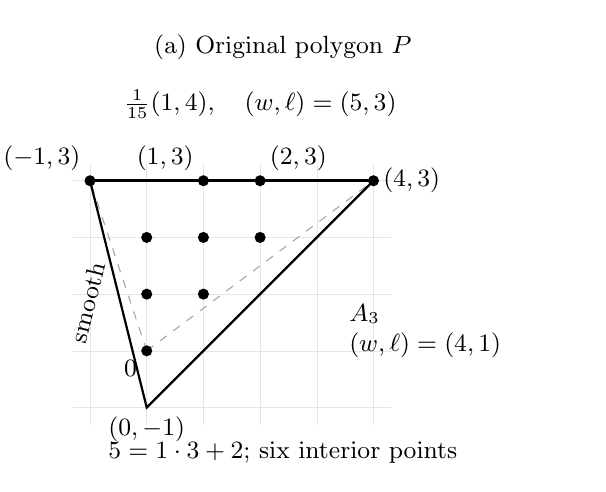
\begin{tikzpicture}[x=0.72cm,y=0.72cm,font=\small]
  \useasboundingbox (-2.1,-2) rectangle (7.6,5.7);
  \node at (2.4,5.35) {(a) Original polygon $P$};
  \draw[step=1,gray!20,very thin] (-1.3,-1.3) grid (4.3,3.3);
  \draw[gray!70,dashed] (0,0)--(-1,3) (0,0)--(4,3);
  \draw[thick] (-1,3)--(4,3)--(0,-1)--cycle;
  \draw[line width=1.1pt] (-1,3)--(4,3);
  \foreach \horizontal/\vertical in {0/0,0/1,0/2,1/1,1/2,2/2}
    \fill (\horizontal,\vertical) circle (2pt);
  \foreach \horizontal in {-1,1,2,4}
    \fill (\horizontal,3) circle (2pt);
  \node[above left] at (-1,3) {$(-1,3)$};
  \node[above left] at (1,3) {$(1,3)$};
  \node[above right] at (2,3) {$(2,3)$};
  \node[right] at (4,3) {$(4,3)$};
  \node[below] at (0,-1) {$(0,-1)$};
  \node[below left] at (0,0) {$0$};
  \node at (2,4.35) {$\frac1{15}(1,4),\quad(w,\ell)=(5,3)$};
  \node[align=left,anchor=west] at (3.4,0.35) {$A_3$\\$(w,\ell)=(4,1)$};
  \node[rotate=76] at (-1.05,0.85) {smooth};
  \node at (2.4,-1.8) {$5=1\cdot3+2$; six interior points};
\end{tikzpicture}
\end{minipage}\hfill
\begin{minipage}[t]{0.49\textwidth}
\centering
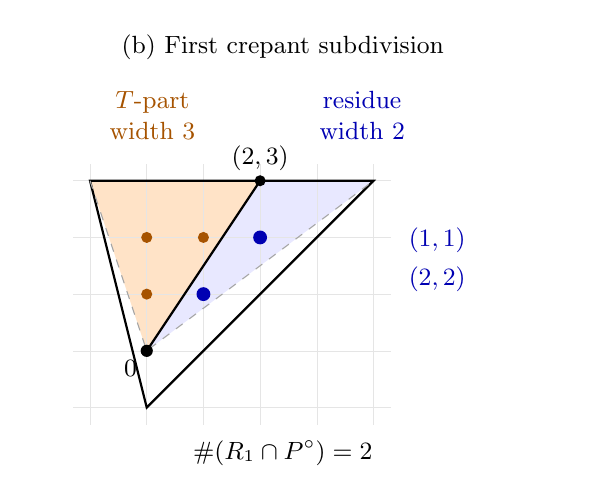
\begin{tikzpicture}[x=0.72cm,y=0.72cm,font=\small]
  \useasboundingbox (-2.1,-2) rectangle (7.6,5.7);
  \node at (2.4,5.35) {(b) First crepant subdivision};
  \fill[orange!22] (0,0)--(-1,3)--(2,3)--cycle;
  \fill[blue!9] (0,0)--(2,3)--(4,3)--cycle;
  \draw[step=1,gray!20,very thin] (-1.3,-1.3) grid (4.3,3.3);
  \draw[thick] (-1,3)--(4,3)--(0,-1)--cycle;
  \draw[gray!70,dashed] (-1,3)--(0,0)--(4,3);
  \draw[thick] (0,0)--(2,3);
  \foreach \horizontal/\vertical in {0/1,0/2,1/2}
    \fill[orange!65!black] (\horizontal,\vertical) circle (2pt);
  \foreach \horizontal/\vertical in {1/1,2/2}
    \fill[blue!70!black] (\horizontal,\vertical) circle (2.5pt);
  \fill (0,0) circle (2.2pt) node[below left] {$0$};
  \fill (2,3) circle (2pt) node[above] {$(2,3)$};
  \node[text=orange!65!black,align=center] at (0.1,4.15) {$T$-part\\width $3$};
  \node[text=blue!70!black,align=center] at (3.8,4.15) {residue\\width $2$};
  \node[text=blue!70!black,anchor=west,align=left] at (4.45,1.6) {$(1,1)$\\[3pt]$(2,2)$};
  \node at (2.4,-1.8) {$\#(R_1\cap P^\circ)=2$};
\end{tikzpicture}
\end{minipage}

\medskip
\begin{minipage}[t]{0.49\textwidth}
\centering
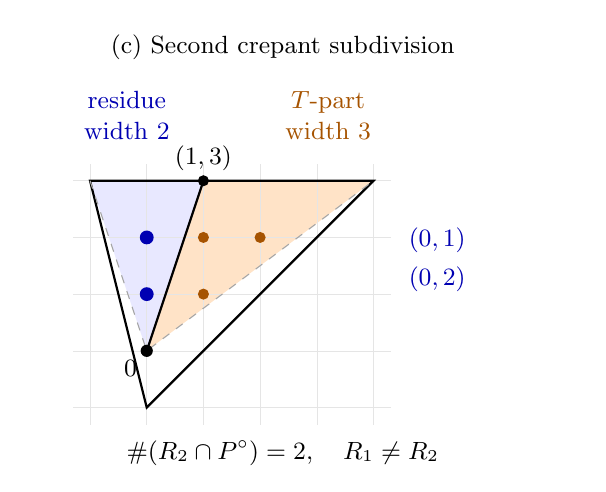
\begin{tikzpicture}[x=0.72cm,y=0.72cm,font=\small]
  \useasboundingbox (-2.1,-2) rectangle (7.6,5.7);
  \node at (2.4,5.35) {(c) Second crepant subdivision};
  \fill[blue!9] (0,0)--(-1,3)--(1,3)--cycle;
  \fill[orange!22] (0,0)--(1,3)--(4,3)--cycle;
  \draw[step=1,gray!20,very thin] (-1.3,-1.3) grid (4.3,3.3);
  \draw[thick] (-1,3)--(4,3)--(0,-1)--cycle;
  \draw[gray!70,dashed] (-1,3)--(0,0)--(4,3);
  \draw[thick] (0,0)--(1,3);
  \foreach \horizontal/\vertical in {1/1,1/2,2/2}
    \fill[orange!65!black] (\horizontal,\vertical) circle (2pt);
  \foreach \vertical in {1,2}
    \fill[blue!70!black] (0,\vertical) circle (2.5pt);
  \fill (0,0) circle (2.2pt) node[below left] {$0$};
  \fill (1,3) circle (2pt) node[above] {$(1,3)$};
  \node[text=blue!70!black,align=center] at (-0.35,4.15) {residue\\width $2$};
  \node[text=orange!65!black,align=center] at (3.2,4.15) {$T$-part\\width $3$};
  \node[text=blue!70!black,anchor=west,align=left] at (4.45,1.6) {$(0,1)$\\[3pt]$(0,2)$};
  \node at (2.4,-1.8) {$\#(R_2\cap P^\circ)=2,\quad R_1\ne R_2$};
\end{tikzpicture}
\end{minipage}\hfill
\begin{minipage}[t]{0.49\textwidth}
\centering
\begin{tikzpicture}[x=1cm,y=1cm,font=\small]
  \useasboundingbox (-1.3,-1.44) rectangle (5.68,4.1);
  \node at (2.15,3.85) {(d) Mutation and lattice equivalence};
  \node at (0,3.1) {$P\rightsquigarrow P'$};
  \begin{scope}[x=0.48cm,y=0.48cm,yshift=0.4cm]
    \draw[step=1,gray!20,very thin] (-1.2,-1.2) grid (1.2,3.2);
    \draw[thick] (-1,3)--(1,3)--(1,-1)--(0,-1)--cycle;
    \foreach \horizontal/\vertical in {-1/3,1/3,1/-1,0/-1}
      \fill (\horizontal,\vertical) circle (1.8pt);
    \node[above left] at (-1,3) {$(-1,3)$};
    \node[above right] at (1,3) {$(1,3)$};
    \node[below right] at (1,-1) {$(1,-1)$};
    \node[below left] at (0,-1) {$(0,-1)$};
  \end{scope}
  \draw[->,thick] (1.05,1.65)--(2.35,1.65) node[midway,above] {$M$};
  \begin{scope}[x=0.48cm,y=0.48cm,xshift=3.7cm,yshift=0.4cm]
    \draw[step=1,gray!20,very thin] (-1.2,-1.2) grid (1.2,6.2);
    \draw[thick] (1,0)--(0,-1)--(-1,2)--(-1,6)--cycle;
    \foreach \horizontal/\vertical in {1/0,0/-1,-1/2,-1/6}
      \fill (\horizontal,\vertical) circle (1.8pt);
    \node[right] at (1,0) {$(1,0)$};
    \node[below] at (0,-1) {$(0,-1)$};
    \node[left] at (-1,2) {$(-1,2)$};
    \node[left] at (-1,6) {$(-1,6)$};
    \node[right] at (0.25,4.8) {$P_6^{(4)}$};
  \end{scope}
  \node at (2.15,-1) {$M=\begin{pmatrix}-1&0\\3&1\end{pmatrix}$};
\end{tikzpicture}
\end{minipage}

\smallskip
{\small
\[
\boxed{(g_{\mathrm{cat}},g_{\mathrm{cat}}^{\mathrm{qG}},g_{\mathrm{MMLP}})=(6,3,3)},
\qquad 6\xrightarrow[\delta=3]{T\text{-content}}3=3.
\]
}